\documentclass[11pt,a4paper]{report} 
\usepackage[utf8]{inputenc} 
\usepackage[norsk]{babel} 
\usepackage{lipsum}

\begin{document}
\title{
Refleksjonsnotat \\
\vspace{2cm}
Aktiv Student - En digital plattform for synliggjøring og kontakt med frivillige organisasjoner\\
Gruppe nr BO20-G06
}

\maketitle

\section*{Eget bidrag - Anders Walle Pettersen}
Jobbet mye med skisser, både lage de og skrive om de. mest ansvar når det ble lagd skisser i Adobe XD. jobbet med brukerundersøkelser, utarbeide spørsmål og jobbe med resultatet. jeg har jobbet litt overalt i dokumentet. 

jeg føler at jeg har jobbet godt. bidratt der jeg kan og der gruppen har trengt meg. gjort alt jeg har fått ansvar for og hjulpet til når de andre har trengt det. jeg føler at jeg har brukt tiden veldig effektivt når jeg har jobbet. 


\section*{Eget bidrag - Ingrid Elise Dahl}

Kort beskrivelse av hva du har gjort, hva slags rolle du har hatt (f.eks. prosjektleder), om det er noe du har hatt spesielt ansvar for, og hvor mye tid du har  brukt.

Evaluering av eget bidrag: Hvordan fungerte du i gruppa? Hva synes du var ditt mest verdifulle bidrag (hva gjorde du best)? Var det noe du kunne gjort bedre? Hva var det viktigste utbytte ditt (hva lærte du mest av)? 

\section*{Eget bidrag - Markus Arnø Madsen}

Min rolle i gruppen har vært kommunikasjons ansvarlig mellom gruppen, veileder og oppdragsgiver, hvor jeg i denne rollen har ordnet med møter og samarbeid mellom alle partene.

Utover min rolle har jeg jobbet mye med sleve skrivingen av hoveddokumentet, utført brukerundersøkelser, lest og skrevet om faglitteratur og hatt mye ansvar i diskusjons kapittelet.
mine hovedbidrag til oppgaven har vært markedsførings kunskap, videre arbeid og anbefalinger + produsering av en del innhold i hoveddokumentet.


Evaluering av eget bidrag:

Jeg synes jeg har fungert godt i gruppen og har fått frem mye av det jeg kan gjennom denne oppgaven. Selv ønsker jeg at jeg kanskje hadde tatt mer ansvar under den tiden hvor vi som gruppe kanskje var litt  lite effektive, men dette løste seg på en bra måte uansett. mitt mest verdifulle bidrag vil jeg si er markedsførings, synlighets og vidre utviklingstipsene som jeg har skrevet i diskusjons kapittelet. jeg er meget stolt og fornøyd med det jeg og gruppen har produsert og håper dette holder til en toppkarakter som er det målet vi satt os ved starten av bachelor perioden.

\section*{Eget bidrag - Stefan Larsen}

Kort beskrivelse av hva du har gjort, hva slags rolle du har hatt (f.eks. prosjektleder), om det er noe du har hatt spesielt ansvar for, og hvor mye tid du har  brukt.

Evaluering av eget bidrag: Hvordan fungerte du i gruppa? Hva synes du var ditt mest verdifulle bidrag (hva gjorde du best)? Var det noe du kunne gjort bedre? Hva var det viktigste utbytte ditt (hva lærte du mest av)? 

\section{Beskrivelse av arbeidsprosessen}

\subsection{Hvordan Covid-19 har påvirket prosjektet}

Som hele verden har merket har vi blitt kraftig rammet av viruset Covid-19. dette har påvirket hele verden i stor grad hvor mange land har stengt helt ned, deriblant dem, Norge.

Dette viruset har ført til begrenset menneskelig kontakt og har også rammet vårt prosjekt og dets planer. Utviklingen av dette produktet vanligvis ville krevd menneskelig samhandling, brukertesting og oversyn fra veiledere, oppdragsgivere og andre fagpersoner.

\subsection{Hva har blitt endret som effekt av viruset?}

Gruppens kontakt med omverdenen og andre mennesker og hverandre har blitt redusert. På grunn av dette har gruppen måtte jobbet alternativt når det kommer til brukertesting og hvordan få input og tilbakemeldinger fra brukerene. Den vanlige arbeidsmåten ved å møtes og skisse, planlegge og snakke sammen, har måtte blitt byttet ut med digitale verktøy for å gjennomføre dette.

\subsection{Hvordan vi har løst dette?}

Gruppen har løst situasjonen ved å ta ibruk digitale verktøy som substitutter for hvordan det ville sett ut uten Covid-19. Dette innebærer bruk av skisserings verktøy som adobe ilustrator, Lucidchart, prototypingsverktøy i form av adobe XD, og digitale kommunikasjonsverktøy som Teams, skype, zoom og discord. 

\subsection{Arbeidsfordeling og tidslinje}

\begin{figure}[H]
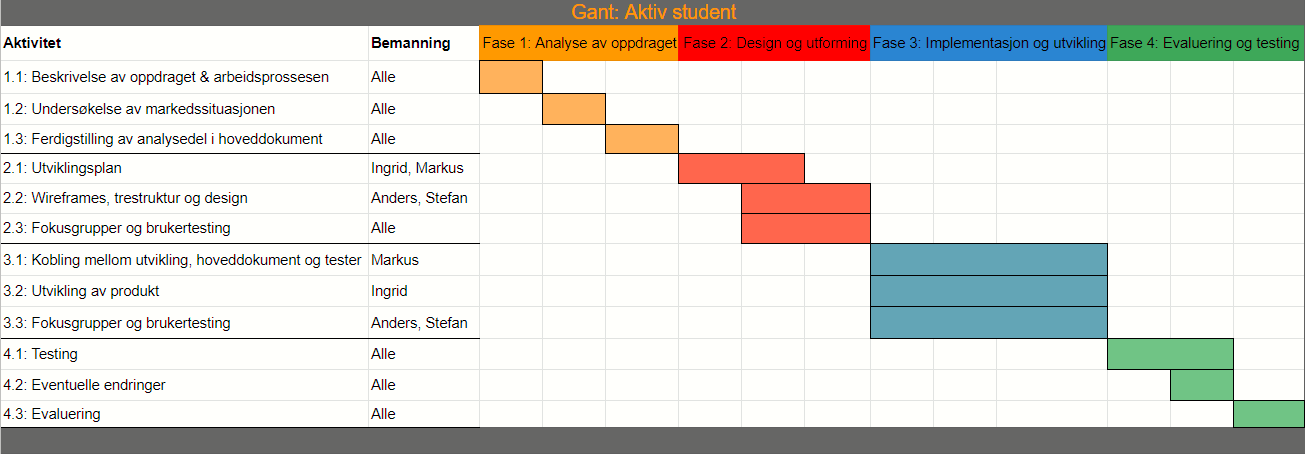
\includegraphics[width=\textwidth]{Illustrasjoner/Gantt.png}
\caption{Gantt-diagram som beskriver oppgaver som skal gjøres og bemanning på de forskjellige delene av prosjektet}
\label{fig:Gantt}
\end{figure}

Gantt diagrammet i figur~\ref{fig:Gantt} er laget for å illustrere de forskjellige hoved-arbeidsoppgavene som må gjennomføres i prosjektet. Diagrammet beskriver punktvis de forskjellige oppgavene som er forklart i hver sin fase av hoveddokumentet og hvilke gruppemedlemmer som har hatt hovedansvar for disse. Gantt-diagrammets formål er å illustrere arbeidsfordeling og skape en bedre oversikt i prosjektet.   

\begin{figure}[H]
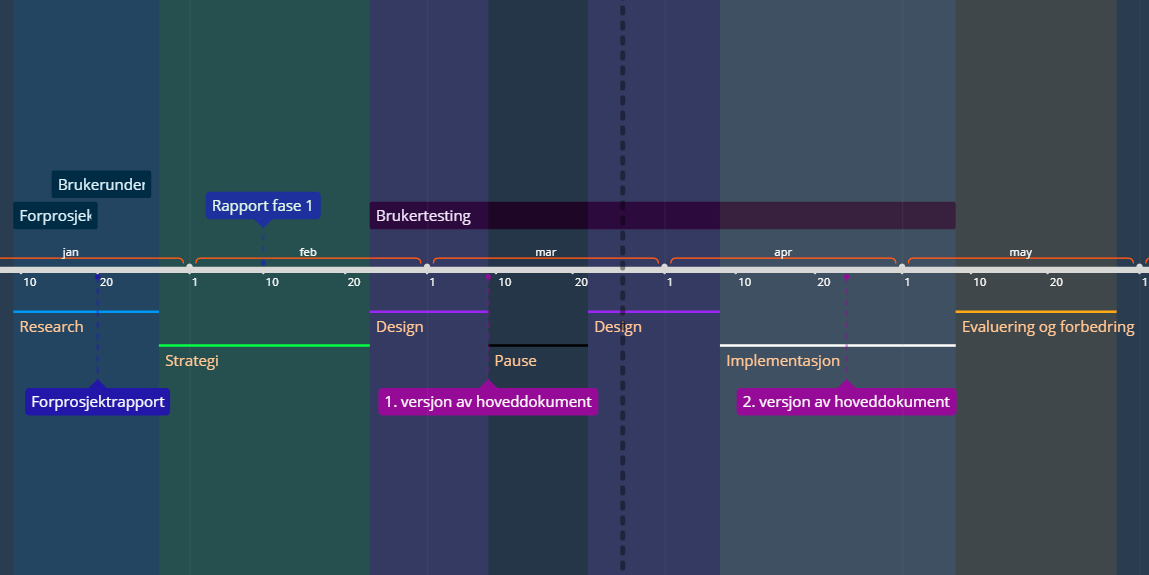
\includegraphics[width=\textwidth]{Illustrasjoner/tidslinje-revidert-igjen.png}
\caption{Tidslinje over prosjektarbeidet}
\label{fig:tidslinje}
\end{figure}

Tidslinjen i figur~\ref{fig:tidslinje} illustrerer de forskjellige fasene i prosjektet og når prosjektgruppen planla å gjennomføre disse. Her vises det at de fem fasene i Informasjonsarkitektur: research, strategi, design, implementasjon og evaluering \& forbedring, er brukt som grunnlag for strukturering av prosjektarbeidet. Viktige frister i løpet av prosjektet er også lagt inn i tidslinjen. 

I ettertid har vi innsett at tidslinjen vi satte var litt for stram, ettersom noen av fasene tok lengre tid enn det som er vist i tidslinjen. Fasene ble likevel brukt som grunnlag for arbeidsprosessen og det oppsto ingen problemer på grunn av at vi gikk utenfor datoene i tidslinjen.


\section*{Samarbeid}
\paragraph{Hvordan fungerte gruppearbeidet?}
Det har fungert svært bra, alle har gjennomført det de har fått ansvar for å gjøre. Alle har vært tilgjengelig for å hjelpe om noen spurte om det. Jo lengre tid som gikk bli vi tryggere på både gruppen og arbeidet. Har utviklet veldig gode rutiner i løpet av arbeidet som vil være veldig fint å ta med seg i arbeidslivet. Kommunikasjonen fungerte også veldig bra da rutinene var på plass, det har vært en god tone mellom gruppemedlemmene og ingen har vært negative til at noen endret på arbeidet deres. Alle har hatt et felles mål i løpet av prosjektet som har vært en klar motivasjon for alle i gruppen og alle har jobbet mot dette målet.

\paragraph{Hvordan fungerte samarbeidet med oppdragsgiver og veileder?}
Vi har fått veldig mye godt ut av samarbeidet med oppdragsgiver. Vi har fått stor frihet for løsningen av oppdraget og har brukt denne friheten til å lage en prototype vi har tro på. Det har vært jevnlige møter med oppdragsgiver ved fysisk oppmøte i begynnelsen og gjennom videomøter på Teams etter Covid-19 brøt ut. Oppdragsgiver har vært svært lett å komme i kontakt med og har vært fleksibel med møtetider.

Samarbeidet med veileder har også fungert bra. Vi har hatt møter eller tatt kontakt på punkter i prosessen der vi har trengt hans vurdering på arbeidet generelt eller på spesifikke punkter i oppgaven. Vi har fått svar på de punktene der vi har konsultert med veileder. Veileder har etter gruppens ønske gitt omfattende konstruktiv kritikk for å oppmuntre gruppen for å gjøre en best mulig jobb. 
    
\paragraph{Hva synes du om resultatene, nådde dere målene dere satte dere?}
Vi er alle svært fornøyde med resultatet. Vi føler at vi har oppfylt kravene og enda mer. Resultatet vi kom fram til ble bedre enn det noen av oss kunne ha sett for oss på starten av semesteret, vi nådde alle mål vi hadde satt oss. Vi har løst oppdraget og utfordringer på veien på en god måte og er veldig stolte av resultatene vi kom fram til både i prototypen og i hoveddokumentet.
 

\section*{Konklusjon}
Alt i alt har hele bachelorprosjektet fungert bra. Selv om det oppsto utfordringer i forhold til Covid-19 som så ut som det kunne stagnert prosjektet klarte gruppen å jobbe rundt dette ved hjelp av digitale verktøy, god planlegging, rutiner og god kommunikasjon. Dette førte til at vi kom inn i en god arbeidsflyt og fikk produsert skisser og gjennomført brukerundersøkelser effektivt slik at vi kom fram til et resultat vi er veldig fornøyd med og stolte av.

\end{document}
